
\qrchapter{https://forgottenpillar.com/rsc/en-fp-chapter15}{Dk. Kellogg na fundisho la Utatu}


Shida kuu ya mzozo wa Kellogg ilikuwa hisia juu ya \emcap{ubinafsi wa Mungu}, ambazo zilikuwa zinaongoza kutoka kwenye msingi wa imani yetu, ambao Mungu alianzisha katika mwanzo wa kazi yetu. Tumeambiwa kwamba \egwinline{Mambo mengi ya tabia kama hayo yatatokea katika siku zijazo}[Ms137-1903.10; 1903][https://egwwritings.org/read?panels=p9939.17]. Katika kitabu, the Living Temple, tunaona hisia kuhusu \emcap{ubinafsi wa Mungu} na mahali uwepo wake ulipo, ambazo zilikuwa zinaondoka kwenye \emcap{Kanuni za Msingi}. Hatua hii haikupaswa kufanywa kamwe! Lakini tunauliza swali, hatua hii ilikuwa inaelekea wapi? Tutaona uthibitisho kwamba hatua hiyo ilikuwa ikielekea kwenye fundisho la Utatu. Dada White alitabiri kwamba hatua ya Kellogg ingeongoza kwenye Omega wa uzushi. Tunaweza kuona uhusiano kati ya mabishano ya Kellogg na fundisho la Utatu?


Katika sehemu ifuatayo, tunataka kukuonyesha uhusiano kati ya mzozo wa Kellogg na fundisho la Utatu. Ni muhimu kusisitiza kwamba Hekalu Hai haina fundisho hili kama inavyoaminika leo. Tatizo kuu la ufundishaji wa Kellogg ulikuwa ni \textit{kuondoka} kutoka kwa \emcap{Kanuni za Msingi}, ambazo zilikuwa msingi wa imani yetu. Taarifa tutakazowasilisha kwako zinafichua kuwa Dk. Kellogg alihalalisha matendo yake ya kuondoka kutoka kwenye msingi kupitia imani yake katika fundisho la Utatu. Hii si vigumu kuona tunapotambua kwamba \emcap{Kanuni za Msingi} zilikuwa zisizo za Utatu. Lengo letu kuu halitakuwa katika kutambua fundisho la Utatu katika hoja za Kellogg, bali kuelewa tofauti kati ya mafundisho ya Kellogg na mafundisho ya \emcap{Kanuni za Msingi} kuhusu \egwinline{ubinafsi wa Mungu na mahali uwepo Wake ulipo}[SpTB02 51.3; 1903][https://egwwritings.org/read?panels=p417.262]. Katika maneno mengine, ni hatua gani Kellogg alichukua katika kuondoka kwenye msingi wa imani yetu? Mbinu hii inatetewa na Roho ya Unabii na itatusaidia kuepukana na mawazo kuhusu nia za Kellogg—itatusaidia kuzingatia ukweli. Ellen White anatuambia kwamba kuna mambo mengi mazuri yaliyoandikwa katika Hekalu Hai, lakini yamechanganyikana na nadharia za udanganyifu na za uongo kuhusu \emcap{ubinafsi wa Mungu} na \emcap{wa Kristo}.



\begin{figure}[hp]
    \centering
    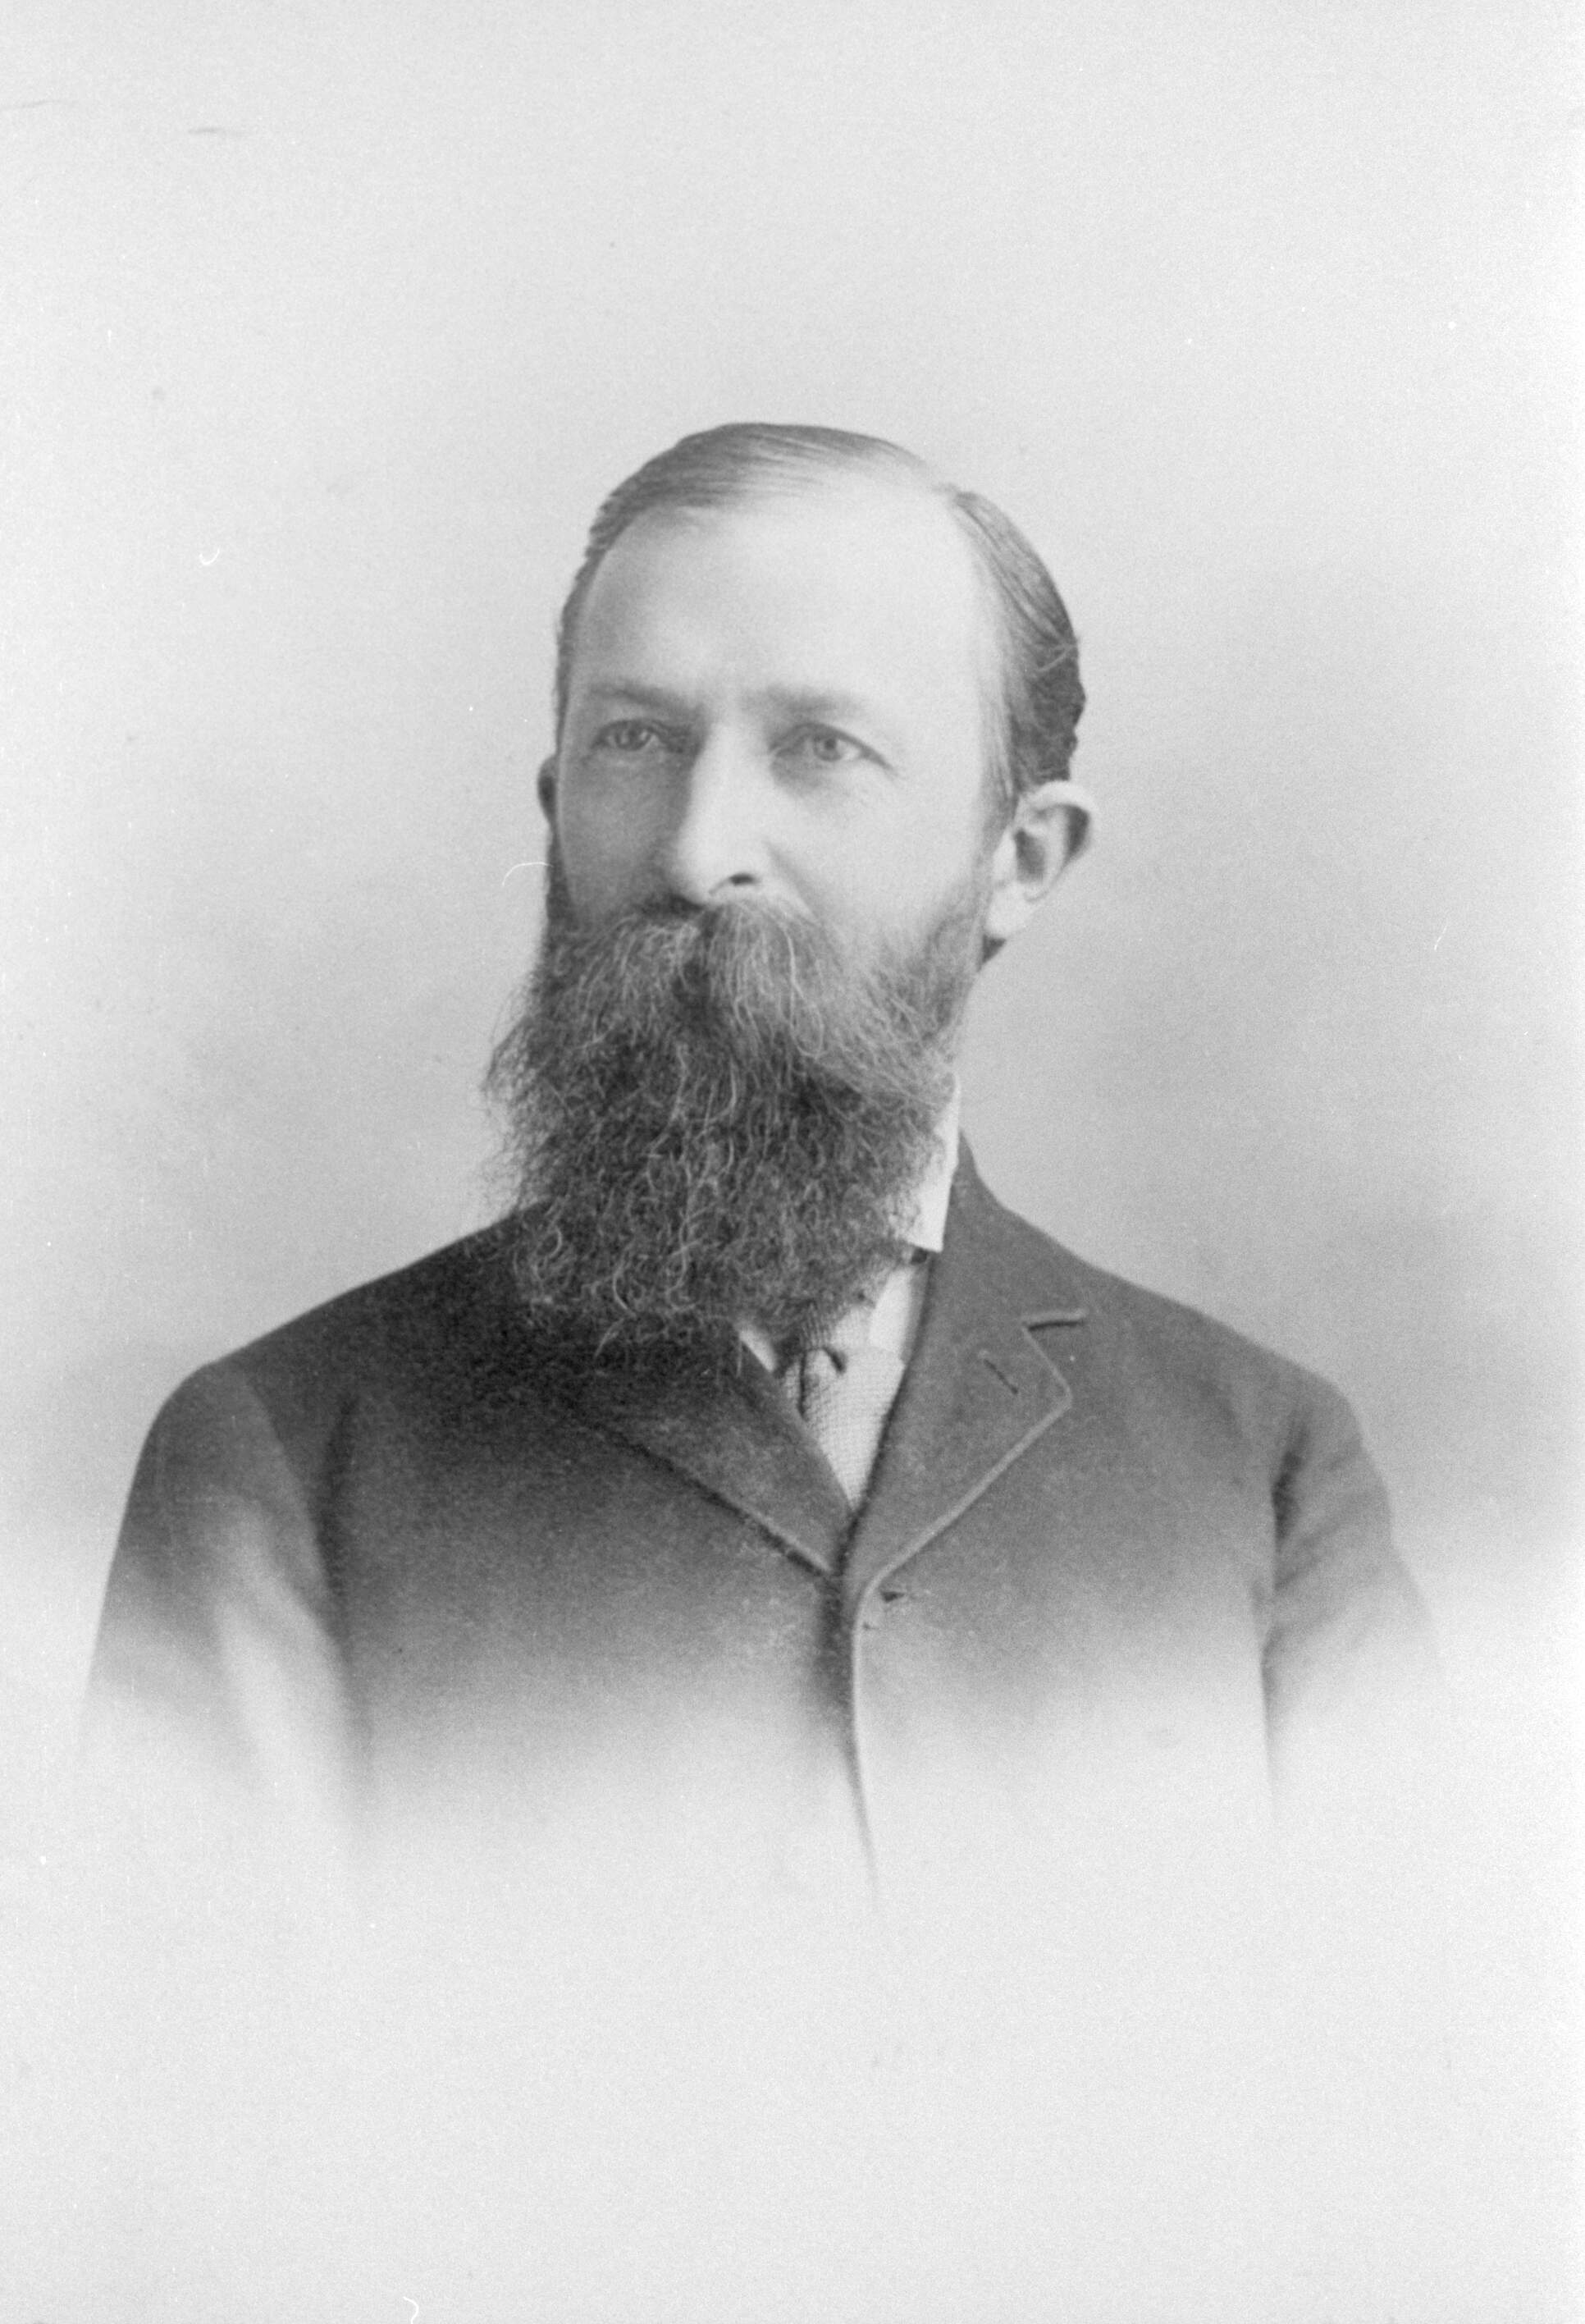
\includegraphics[width=1\linewidth]{images/john-h-kellogg.jpg}
    \caption*{John Harvey Kellogg (1852-1943)}
    \label{fig:john-h-kellogg}
\end{figure}


\egw{\textbf{Kitabu Hekalu Hai kina maoni ya uwongo, \underline{ya udanganyifu kuhusu ubinafsi wa Mungu na wa Kristo}}. Bwana alifungua mbele yangu maana halisi ya hisia hizi, akinionyesha kwamba ikiwa mafundisho haya hayatakataliwa kwa uthabiti, yanaweza kuwapoteza, kama yamkini, hata walio wateule. \textbf{Ukweli wa thamani na hisia nzuri ziliunganishwa na uwongo, nadharia potofu. Hivyo ukweli ulitumiwa kuthibitisha \underline{makosa ya hatari zaidi}. Vielelezo vya thamani vya Mungu vimefafanuliwa vibaya sana hivi kwamba vinaonekana kuunga mkono udanganyifu \underline{ulioasisiwa na yule muasi mkuu}. Hisia ambazo ni za ufunuo ya Mungu zimechanganyika na nadharia zenye udanganyifu za mashirika ya kishetani}.}[Lt146-1905.2; 1905][https://egwwritings.org/read?panels=p9430.8]


\egwnogap{Katika mabishano ya nadharia hizi \textbf{imedaiwa kwamba niliamini na kufundisha mambo yale yale} ambayo nimeagizwa kukemea katika kitabu Hekalu Hai. \textbf{Hili ninakataa}. Kwa jina la Yesu Kristo wa Nazareti, \textbf{nasema sivyo hivyo}.}[Lt146-1905.3; 1905][https://egwwritings.org/read?panels=p9430.9]


Mchanganyiko huu wa ukweli na makosa hufanya jambo kuwa gumu. Katika macho ya wataalamu wanaounga mkono utatu, tatizo linahusishwa tu na pantheism, na ushahidi wa imani ya Kellogg katika fundisho la Utatu linafasiriwa kuwa imani katika Utatu wa uwongo\footnote{Whidden, Woodrow W, et al. \textit{The Trinity : Understanding God's Love, His Plan of Salvation, and Christian Relationships}. Hagerstown, Md, Review And Herald Pub. Association, 2002., p. 217}. Karipio la Dada White linahusishwa na utetezi wa Utatu “sahihi,” ambao inasemekana aliamini. Kwa bahati mbaya, tafsiri kama hiyo haihusishi utetezi wa Dada White wa \emcap{Kanuni za Msingi} kuhusu \emcap{ubinafsi wa Mungu} na wa Kristo, hivyo ni tafsiri mbaya ya kazi yake. Katika sehemu zifuatazo, tutaangalia data ya kihistoria kuhusu uhusiano wa Dk. Kellogg na fundisho la Utatu kutoka kwa mtazamo wa ukweli wa Waadventista juu ya \emcap{ubinafsi wa Mungu}, ambao ulikuwa msingi wa imani yetu. Tukiwa na mtazamo huu, tunaamini kwamba data ya kihistoria itaangaza katika mwanga mpya na kuibua mazungumzo ya uaminifu na yenye kujenga katika kanisa letu.



\section*{Mawasiliano ya Dk. Kellogg na Ndugu Butler}


Katika sehemu ifuatayo tunawasilisha kwa ufupi mawasiliano yanayojulikana kati ya Dk. Kellogg na G. I. Butler juu ya kitabu, the Living Temple. Hapa, tunaona pingamizi ya Dk. Kellogg kuhusu mzozo huo. Alimwandikia Ndugu Butler:


\others{Kadiri ninavyoweza kufahamu, \textbf{utata} unaopatikana \textbf{katika ‘The Living Temple’,} \textbf{kwa ujumla jambo linaweza kuchemshwa hadi kwenye swali}: \textbf{\underline{Je, Roho Mtakatifu ni nafsi}?} Unasema hapana. Nilidhani kwamba Biblia ilisema hivi kwa sababu kiwakilishi cha kibinafsi ‘yeye’ kinatumika akizungumza juu ya Roho Mtakatifu. \textbf{Dada White anatumia kiwakilishi ‘yeye’ na amesema katika maneno mengi sana kwamba Roho Mtakatifu ni \underline{nafsi ya tatu ya Uungu}}. \textbf{Jinsi Roho Mtakatifu anaweza kuwa nafsi ya tatu na asiwe nafsi hata kidogo ni vigumu kwangu kuona}.}[Letter: J. H. Kellogg to G. I. Butler. Oct 28. 1903][https://static1.squarespace.com/static/554c4998e4b04e89ea0c4073/t/5db9fbc96defed1e45b497a4/1572469707862/1903-10-28-Kellog-to-Butler.pdf]


\begin{figure}[hp]
    \centering
    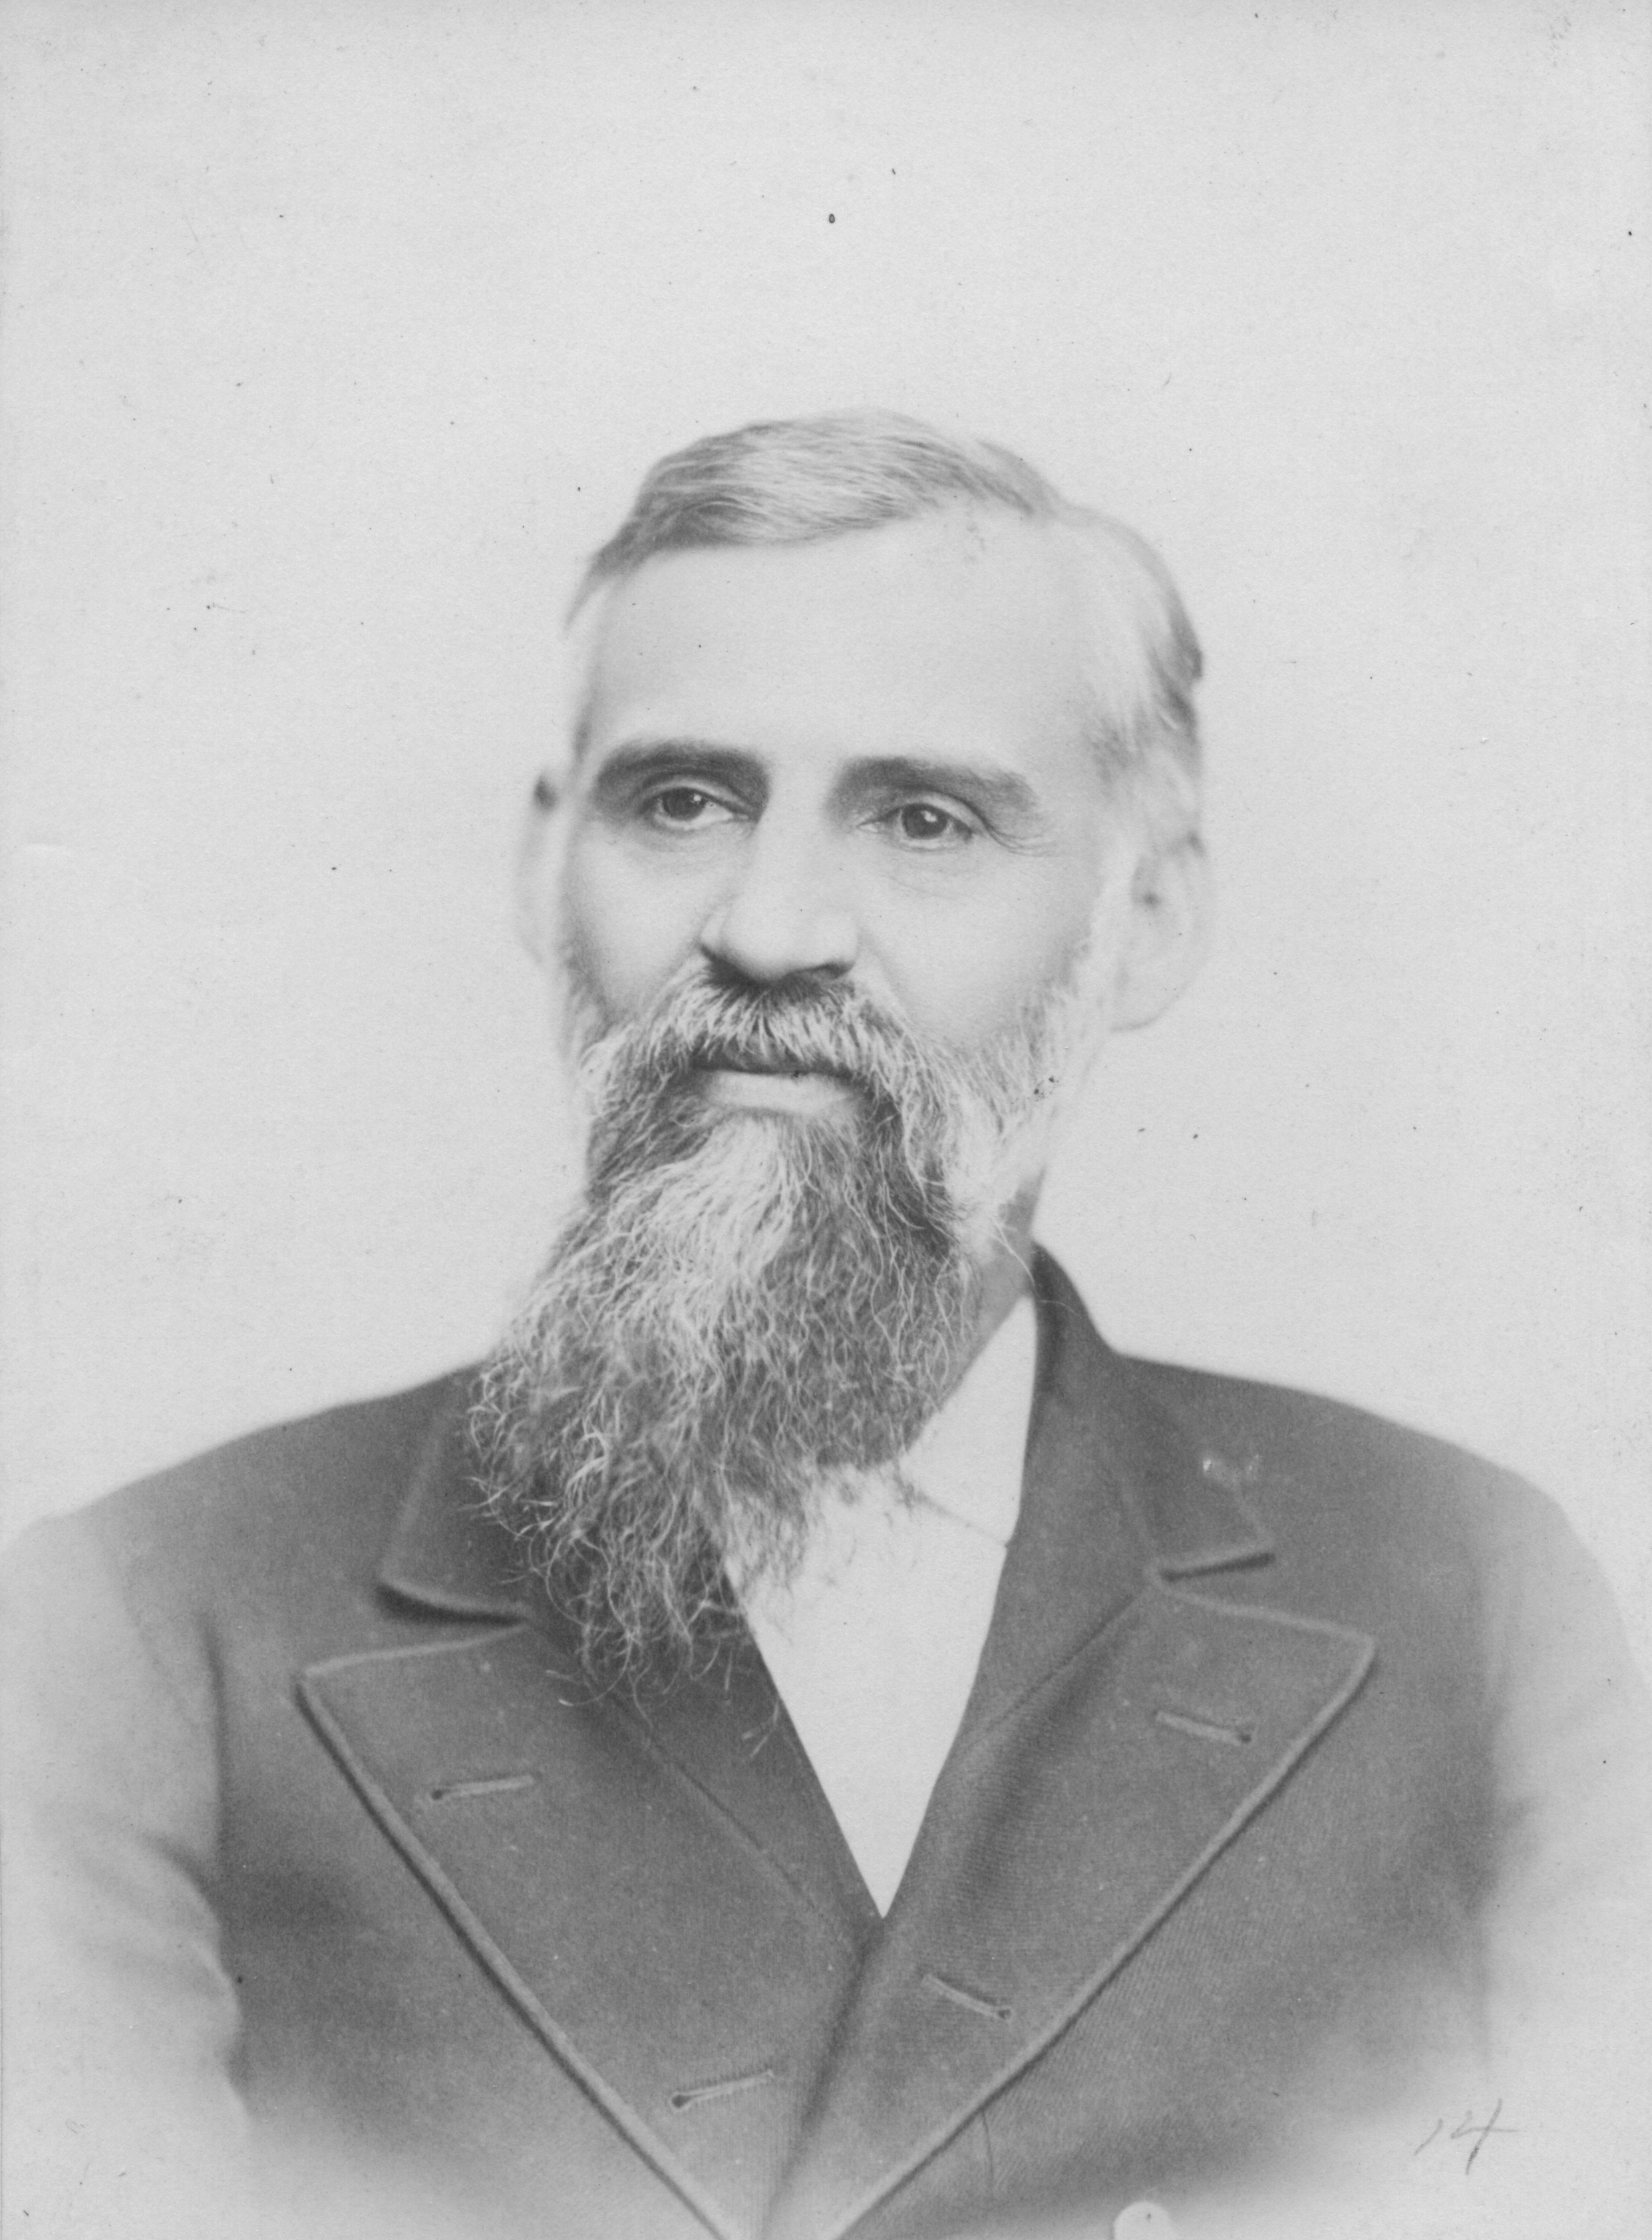
\includegraphics[width=1\linewidth]{images/george-ide-butler.jpg}
    \caption*{George Ide Butler (1834-1918)}
    \label{fig:g-i-butler}
\end{figure}


Kulingana na mtazamo wa Dk. Kellogg, tatizo zima la kitabu ‘The Living Temple’ inakuja kwa swali “\textit{Je! Roho Mtakatifu ni nafsi?}”. Ni wazi, yeye hatetei Mungu asiye na nafsi, kama anavyoshutumiwa mara nyingi\footnote{Whidden, Woodrow W, et al. \textit{The Trinity : Understanding God's Love, His Plan of Salvation, and Christian Relationships}. Hagerstown, Md, Review And Herald Pub. Association, 2002., p. 217}. Zaidi ya hayo, hata anaamini kwamba Roho Mtakatifu ni \textit{nafsi ya tatu ya Uungu}. Pia, anadai kwamba Ndugu Butler haamini kwamba Roho Mtakatifu ni nafsi. Tatizo ni wazi liko katika ufafanuzi wa neno \textit{‘nafsi’}. Katika hatua hii, Kellogg anaendelea:


\others{Ninaamini huyu Roho wa Mungu kuwa nafsi wewe huamini. Lakini hili ni swali tu la ufafanuzi. \textbf{Ninaamini Roho wa Mungu ni nafsi}; unasema, Hapana, sio nafsi. Sasa sababu pekee kwa nini tunatofautiana ni kwa sababu \textbf{tunatofautiana katika mawazo yetu kuhusu \underline{nini ni nafsi}}. \textbf{Wazo lako la nafsi labda ni la \underline{kufanana na mtu} au na binadamu}.}[Letter: J. H. Kellogg to G. I. Butler. Oct 28. 1903][https://static1.squarespace.com/static/554c4998e4b04e89ea0c4073/t/5db9fbc96defed1e45b497a4/1572469707862/1903-10-28-Kellog-to-Butler.pdf]


Ndugu Butler alijibu:


\others{\textbf{Ikiwa Dada White na wewe mko katika makubaliano kamili, itabidi niachane na hilo swala kabisa liwe kati yako na Dada White. \underline{Dada White anasema hakuna makubaliano kamilifu; unadai ipo}. \underline{Najua baadhi ya maandishi yake yanaonekana kukupa nguvu katika kudai kuwa anafanya hivyo}. Niko wazi vya kutosha kusema hivyo, lakini lazima nimpe nafasi yake mpaka akanushe kwa kusema kuna tofauti pia, na siamini unaweza kusema kikamilifu kile anachomaanisha. \underline{Mungu anakaa ndani yetu kwa Roho wake Mtakatifu}, kama Mfariji, kama Mkemeaji, hasa yule wa kwanza. Tunapokuja Kwake tunamshiriki yeye kwa sababu Roho hutoka Kwake; \underline{inatoka kwa Baba na Mwana}. Si nafsi anayetembea kwa miguu, au kuruka \underline{kama huluki halisi}, \underline{kwa maana yoyote kama Kristo na Baba walivyo} - angalau, ikiwa ni hivyo, ni zaidi ya ufahamu wangu wa maana ya lugha au maneno}.}[Letter: G. I. Butler to J. H. Kellogg. April 5. 1904]


Mawasiliano yaliyotolewa ni muhimu kwa kuelewa mgogoro wa Kellogg. Kellogg mwenyewe alisema, \others{jambo zima linaweza kuchambuliwa hadi kukifikia kiini chake kwa swali: \textbf{Je, Roho Mtakatifu ni nafsi?}} Vivyo hivyo Dk. Kellogg alimwandikia William White: \others{Nimekuwa nikisoma kwa makini sana kuona \textbf{ni nini kiini cha tatizo la Hekalu Hai}, na kadiri ninavyoweza kuona \textbf{\underline{swali zima} linajikita katika hili: \underline{Je, Roho Mtakatifu ni nafsi}?}}[Letter J. H. Kellogg to William White, October 28, 1903][https://drive.google.com/file/d/1\_S4S-Hc0K7Ka8gda9oRhPuAb9XzBTwmb/view] Je! hitimisho la Kellogg linaendeleaje kulinganishwa na mapitio na maelekezo ya asili ya mbinguni, ambayo yalituambia wazi kwamba mantiki katika Hekalu Hai ni \egwinline{si chochote ila ni dhana tu kuhusiana na \textbf{Umbile la Mungu na mahali uwepo wake ulipo}}[SpTB02 51.3; 1904][https://egwwritings.org/read?panels=p417.262]? Katika maandiko ya Ellen White na waanzilishi, neno ‘\textit{Umbile la Mungu}’ linahusu hasa Umbile la Baba. Kwa hiyo, kwa nini Kellogg anadai kwamba suala halisi ni Umbile la Roho Mtakatifu, wakati Mungu alionyesha kwamba suala linahusu Umbile la Baba?



Wengi wanadhani kwamba Dk. Kellogg anajaribu kudanganya, akikwepa suala la msingi. Hata hivyo, chini ya dhana fulani, hoja zake kuhusu Umbile la Roho Mtakatifu kimatiki zinaunga mkono maoni yake ya utata kuhusu \emcap{Umbile la Mungu}. Dhana hii inakuwa dhahiri ndani ya data yenyewe tunapofuata kwa makini mantiki yake.


Kama tulivyoona hapo awali, fundisho juu ya \emcap{Umbile la Mungu} linafundisha kwamba Mungu, Baba, ana umbo—mwili unaoonekana, wa dutu. Dk. Kellogg alikubali kwamba dai hili ni kweli ndani ya mipaka ya uelewa wetu finyu wa Mungu\footnote{\href{https://archive.org/details/J.H.Kellogg.TheLivingTemple1903/page/n33/}{Dr. John H. Kellogg, The Living Temple, p.31.}}. Hata hivyo, alihoji kwamba, kwa kweli, Mungu anazidi dhana zetu kuhusu umbo lake, kwani yuko nje ya vikwazo vya nafasi\footnote{\href{https://archive.org/details/J.H.Kellogg.TheLivingTemple1903/page/n33/}{Dr. John H. Kellogg, The Living Temple, p.33.}}. Kwa maana hii, Kellogg kwa kweli anaondoa uhalisia wa mwili wa kimwili, wa dutu wa Mungu. Dhana ambayo ingethibitisha mtazamo wa Dk. Kellogg ni \textit{ulinganifu wa kipekee} katika kuelewa \emcap{Umbile la Mungu} na lile la Roho Mtakatifu. Je, Roho Mtakatifu anazuiliwa na nafasi? Hapana, hazuiliwi. Je, Roho Mtakatifu ana mwili wa kimwili? Hapana! Kulingana na Yesu, \bible{kwa maana roho haina mwili wala mifupa}[Luka 24:39]. Je, Roho Mtakatifu ni nafsi? Jibu linategemea tafsiri yetu ya maana ya kuwa nafsi. Ni nini ubora au hali ya Roho Mtakatifu kuwa nafsi?\footnote{Matumizi ya moja kwa moja ya ufafanuzi wa neno ‘\textit{Umbile}’ kutoka \href{https://www.merriam-webster.com/dictionary/personality}{Kamusi ya Merriam Webster}} Tunapolinganisha imani ya Dk. Kellogg katika Umbile la Roho Mtakatifu na maoni ya Ndugu Butler, inakuwa dhahiri kwamba ubora wa Roho Mtakatifu kuwa nafsi hauendani na \others{ule wa \textbf{kufanana na mtu} au binadamu}. Butler alieleza wazi vigezo vyake kwa uamuzi huu\footnote{Katika barua yake kwa Dk. Kellogg, Ndugu Butler pia alidai kwamba hakuna tofauti kati ya nafsi na uwepo wa kimwili. Tazama \href{https://c7da.us/egwdl/Butler\%20to\%20Kellogg\%20Aug121904.pdf}{Barua kutoka Butler kwa Kellogg, Agosti 12, 1904, uk.6}}: \others{\textbf{Si nafsi anayetembea kwa miguu, au kuruka \underline{kama huluki halisi}, \underline{kwa maana yoyote kama Kristo na Baba walivyo} - angalau, ikiwa ni hivyo, ni zaidi ya ufahamu wangu wa maana ya lugha au maneno}}.


Je, umeona kwamba Ndugu Butler alishughulikia dhana ya Kellogg ambayo hakusema? Butler aliweka tofauti kati ya Baba na Kristo, kuhusiana na Roho Mtakatifu. Ndugu Butler yuko sahihi. Kuna tofauti kati ya Umbile la Roho Mtakatifu na lile la Mungu na Kristo. Kristo na Baba wana umbo la kimwili la mtu, wakati Roho Mtakatifu hana. Kuondoa umbo la kimwili la nafsi ya Baba ni \textit{kulinganisha kwa kipekee} uelewa wa Umbile la Baba na lile la Roho Mtakatifu. Mtazamo wa Kellogg ni wa kushawishi, kwa sababu uliungwa mkono na hoja halali kuhusu Umbile la Roho Mtakatifu.


Hebu tuchunguze kwa ufupi Umbile la Roho Mtakatifu. Ni nini ubora au hali ya Roho Mtakatifu kuwa nafsi?


\egw{\textbf{Roho Mtakatifu ana Umbile}, \textbf{\underline{vinginevyo} }Asingeweza \textbf{kushuhudia} kwa roho zetu na pamoja na roho zetu kwamba sisi ni watoto wa Mungu. \textbf{Lazima pia awe \underline{Nafsi ya kimungu}}, \textbf{\underline{vinginevyo}} Asingeweza \textbf{kuchunguza siri} zilizofichika \textbf{katika akili ya Mungu}.}[21LtMs, Ms 20, 1906, par. 32; 1906][https://egwwritings.org/read?panels=p14071.10296041&index=0]


\egw{\textbf{Roho Mtakatifu ni nafsi}; \textbf{\underline{kwa}} Yeye \textbf{hushuhudia} pamoja na roho zetu kwamba sisi ni watoto wa Mungu.}[21LtMs, Ms 20, 1906, par. 31; 1906][https://egwwritings.org/read?panels=p14071.10296040&index=0]


Sifa au hali zinazomfafanua Roho Mtakatifu kama nafsi zimetajwa wazi katika nukuu zilizotolewa. Hizi ni pamoja na uwezo wa kushuhudia na kuchunguza akili. Ushahidi zaidi unaweza kupatikana katika Maandiko, ambayo yanampa Roho Mtakatifu matendo kama vile kuzungumza (\textit{Matendo 13:2}), kufundisha (\textit{Yohana 14:26; 1 Wakorintho 2:13}), kufanya maamuzi (\textit{Matendo 15:28}), na kuwa na hisia (\textit{Waefeso 4:30}), miongoni mwa nyingine. Hizi \textit{sifa} kwa pamoja zinathibitisha Umbile la Roho Mtakatifu. Je, sifa hizi zinaweza kutumika pia kwa Baba na Mwana? Bila shaka. Hata hivyo, tofauti na Baba na Mwana, Roho Mtakatifu anatofautishwa kwa kukosa umbo la kimwili, linaloonekana. Wakati Ellen White alipomwuliza Kristo kuhusu \emcap{Umbile la Mungu}, swali lake hasa lililenga umbo la kibinafsi kama sifa inayofafanua Umbile la Baba.


\egw{Mara nyingi \textbf{nimemwona} Yesu mzuri, kwamba \textbf{Yeye ni nafsi}. \textbf{Nilimwuliza kama Baba Yake \underline{alikuwa nafsi} na \underline{alikuwa na umbo} kama Yeye}. Yesu alisema, ‘\textbf{Mimi ni chapa kamili ya Umbile la Baba yangu}.’}[EW 77.1; 1882][https://egwwritings.org/read?panels=p28.490&index=0]


Hii inatuleta kwenye tofauti kubwa katika jinsi Umbile la Roho Mtakatifu linavyoeleweka, tofauti na lile la Baba na Mwana. Ellen White anaelezea Roho Mtakatifu kama dhihirisho la kiroho la Kristo, akiweka mstari wazi kati ya dhihirisho la nje, linaloonekana la Kristo na dhihirisho lake la kiroho. Tofauti hii inasisitiza asili ya kipekee ya uwepo na utendaji wa Roho Mtakatifu duniani, tofauti na uwepo wa kimwili wa Kristo na Baba. Zingatia tofauti kati ya dhihirisho la nje, linaloonekana la Kristo, na dhihirisho lake la kiroho:


\egw{Kwamba \textbf{Kristo} angeweza \textbf{kujidhihirisha} kwao, na bado \textbf{asiwe anaonekana kwa ulimwengu}, ilikuwa siri kwa wanafunzi. Hawakuweza kuelewa \textbf{maneno ya Kristo katika \underline{maana yake ya kiroho}}. \textbf{Walikuwa wanafikiria \underline{dhihirisho la nje, linaloonekana}}. Hawakuweza kuelewa ukweli kwamba wangeweza kuwa na \textbf{uwepo wa Kristo pamoja nao}, na \textbf{bado Yeye asionekane na ulimwengu}. \textbf{Hawakuelewa maana ya \underline{dhihirisho la kiroho}}.}[ST November 18, 1897, par. 6; 1897][https://egwwritings.org/read?panels=p820.14727&index=0]


Roho Mtakatifu si nafsi kwa maana ya kimwili bali anadhihirishwa kwa maana ya kiroho. Ikiwa uelewa wa kipekee wa Umbile la Roho Mtakatifu utatumika kwa Baba, basi kwa matokeo yake umbo lake la kimwili la nafsi linaondolewa. Umbile lake linafanywa kuwa la kiroho. Hii ndiyo sababu Ellen White alitaja mtazamo wa Kellogg kama umizimu. Je, unajua fundisho gani, hasa, lina kanuni kuu, kwamba Baba na Roho Mtakatifu ni sawa katika Umbile lao? Ni \textit{fundisho la utatu}. Je, inawezekana kwamba Dk. Kellogg alikuwa kwa kweli anainua upande wa kitheolojia wa maswali ya utatu?


\section*{Ungamo la Kellogg kuhusu Hekalu Hai}


Katika mahojiano yake na G. W. Amadon na A. C. Bourdeau, mwezi mmoja baada ya kutengwa na ushirika, alikiri kwamba bila kukusudia alileta upande wa kitheolojia wa swali la Utatu katika kitabu chake “The Living Temple”.


\others{\textbf{Sasa, nilifikiri nilikuwa nimeondoa kabisa upande wa kitheolojia wa maswali ya \underline{utatu na aina hiyo ya mambo}}. \textbf{Sikukusudia \underline{kuiweka ndani} hata kidogo}, na nilichukua tahadhari kueleza katika dibaji kwamba sikufanya hivyo. Sikuwahi kufikiri chochote kuhusu \textbf{swali lolote la kitheolojia} \textbf{\underline{kuletwa ndani yake}}. Nilitaka tu kuonyesha kwamba \textbf{moyo haupigi kwa mwendo wake bali kwamba ni uweza wa Mungu unaoufanya uendelee}.}[Kellogg vs. The Brethren: His Last Interview as an Adventist, p. 58.][https://forgotten-pillar.s3.us-east-2.amazonaws.com/1990\_kellogg\_vs\_brethren\_lastInterview\_oct7\_1907\_spectrum\_v20\_n3-4.pdf]


Kama tungetafuta katika kitabu chake maneno ya utatu, hatungepata yoyote. Je! hilo lingekuwa ushahidi kwamba Kellogg hana ufahamu katika kukiri kwake? Kitu pekee tunachopata ni mafundisho ambayo yanaondoka kutoka kwenye msingi wa imani yetu—\emcap{kanuni za kimsingi}—kuhusu \emcap{ubinafsi wa Mungu} na mahali uwepo wake ulipo. Semi za utatu hazipo hapo bali hisia zake kuhusu \emcap{ubinafsi wa Mungu} zinapatana na hisia za utatu kuhusu ubinafsi wa Mungu. Hisia hizi ni za udanganyifu na Kellogg alikemewa kwayo. Alipotaka kueleza kwa uwazi imani katika fundisho la Utatu, kwa matumaini ya kurekebisha kitabu, alikemewa tena kwa maneno, \egwinline{\textbf{Nadharia za kiraka} haziwezi kukubaliwa na wale walio waaminifu kwa imani} na kwa \emcap{Kanuni za Msingi}\footnote{\href{https://egwwritings.org/?ref=en_Lt253-1903.28&para=9980.36}{EGW, Lt253-1903.28; 1903}}. Tatizo la muhimu la fundisho la Utatu, kuhusiana na \emcap{ubinafsi wa Mungu}, ndilo dhana ya msingi ambayo wote Tatu, Baba, Mwana, na Roho Mtakatifu, wana aina moja ya ubinafsi hivi kwamba Hao hujumuisha Mungu mmoja. Katika mwanga huu, tunaweza kuelewa madai ya Kellogg juu ya ubinafsi wa Roho Mtakatifu, kwamba Roho Mtakatifu ni nafsi ya tatu ya Uungu. Dk. Kellogg alimnukuu Ellen White wakati akisisitiza madai yake; ingawa alitumia maneno sawa, alikuwa na hisia mbaya. Kwa kuzingatia kukiri kwa Dk. Kellogg, kwa kujumuisha \others{\textbf{upande wa kitheolojia wa maswali ya \underline{utatu}}}, na madai yake kwamba \others{\textbf{jambo zima inaweza kuchambuliwa hadi swali}: \textbf{\underline{Je, Roho Mtakatifu ni nafsi}}?}, tunaweza kuona dhana fiche kwamba Baba na Mwana ni Nafsi kwa njia sawa na Roho Mtakatifu. Hii ndiyo sababu Ndugu Butler alimwandikia kuhusu ubinafsi wa Roho Mtakatifu: \others{\textbf{Siyo Nafsi anayetembea kwa miguu, au kuruka \underline{kama huluki halisi}, \underline{sawia na jinsi Kristo na Baba walivyo} – angalau, ikiwa ni, ni zaidi ya ufahamu wangu ya maana ya lugha au maneno.}}[Letter from G. I. Butler to J. H. Kellogg, April 5 1904.]


\section*{Uwepo wa Mungu unadhihirika katika asili}


Kutoka kwa kazi za waanzilishi wetu, tumeona kwamba ubinafsi wa Roho Mtakatifu zaidi imeonyeshwa wazi katika suala la uwepo wa Mungu. Dada White alituambia kwamba Hekalu Hai \egwinline{hutanguliza yale ambayo si chochote ila ni dhana tu kuhusiana na \textbf{ubinafsi wa Mungu na mahali ambapo uwepo wake upo}.}[SpTB02 51.3; 1904][https://egwwritings.org/read?panels=p417.262] \emcap{Ubinafsi wa Mungu} na mahali palipo na uwepo wake ni mafundisho mawili yanayojumuisha pande zote; mmoja inathibitisha nyingine. Kataa moja, unakana lingine. Dhana hii inaonekana wazi katika kitabu, Hekalu Hai. Katika sehemu zilizopita, tunasoma hoja za Kellogg za \emcap{ubinafsi wa Mungu} zilizochukuliwa kutoka katika kitabu chake. Alipinga kuwa haina maana kuzungumza kuhusu umbo la Mungu au namna yoyote inayoonekana. Alikana ukweli wa Mungu kama nyenzo iliyo dhahiri na huluki anayeonekana. Ikiwa Mungu ni roho, hana umbo wala mwili, basi hasitiriwi katika uwepo wake kwa eneo moja; Haya ndiyo maoni ambayo Kellogg aliyatetea katika Hekalu Hai.


\others{Mmoja husema, ‘\textbf{Mungu anaweza kuwapo kwa Roho wake, au kwa nguvu zake, lakini \underline{hakika Mungu mwenyewe} hawezi kuwapo kila mahali mara moja kwa wakati mmoja}.’ Tunajibu: Nguvu inaweza kuwaje kutengwa na chanzo cha nguvu? \textbf{Ambapo Roho wa Mungu anafanya kazi}, ambapo kuna nguvu za Mungu iliyodhihirika, \textbf{Mwenyezi Mungu \underline{yumo} na hakika yuko}…}[John H. Kellogg, The Living Temple, p.28.][https://archive.org/details/J.H.Kellogg.TheLivingTemple1903/page/n29/]


Wakati Dk. Kellogg aliandika \others{Anasema mmoja, ‘Mungu anaweza kuwa kwa Roho Wake…‘}, alirejelea hisia za mapainia wetu ambao walikuwa waaminifu kwa \emcap{Kanuni za Msingi}. Hapa ndipo mahali dhahiri ambapo Dk. Kellogg aliondoka kutoka kwenye \emcap{Kanuni za Msingi}. Je, hatua hii inapatana na fundisho la Utatu? Tukichunguza msimamo wetu wa sasa katika Mafundisho za Kimsingi \#2, tunaona kwamba Mungu mmoja, kama umoja wa nafsi tatu, hayupo kila mahali kupitia wakala wa Roho Mtakatifu, bali yupo kila mahali kwa Nafsi yake.


\others{Kuna \textbf{Mungu mmoja}: Baba, Mwana, na Roho Mtakatifu, \textbf{umoja wa} \textbf{Nafsi} tatu zenye umilele sawa. Mungu ni asiyekufa, mwenye nguvu zote… na \textbf{yupo kila mahali}.}[Fundamental Beliefs of Seventh-day Adventist, \#2 Trinity; 2020 Edition][https://www.adventist.org/wp-content/uploads/2020/06/ADV-28Beliefs2020.pdf]


\section*{Mtazamo wa Dk. Kellogg kuhusu Mungu}


Katika kuchunguza mzozo uliozunguka Hekalu Hai, tunaona kweli kwamba Dk. Kellogg aliibua \others{upande wa kitheolojia wa maswali ya utatu.}[Kellogg vs. The Brethren: His Last Interview as an Adventist, p. 58.][https://forgotten-pillar.s3.us-east-2.amazonaws.com/1990\_kellogg\_vs\_brethren\_lastInterview\_oct7\_1907\_spectrum\_v20\_n3-4.pdf] Swali lingine tunaloibua katika kuchunguza hisia za Kellogg na \emcap{Kanuni za Msingi} ni nani anayerejelea kwa maneno “\textit{Mungu mmoja}”? Hakuna data ya kujibu swali hilo moja kwa moja, lakini kuna data nyingi zinazoonyesha kwamba uelewa wa Dk. Kellogg wa “\textit{Mungu mmoja}” ulikuwa uelewa wa Utatu. Barua yake kwa W. W. Prescott ni ushahidi mmoja unaoonyesha dhana hiyo:


\others{Tofauti ni hii: \textbf{Tunaposema Mungu} yumo kwenye mti, neno ‘\textbf{Mungu}’ \textbf{linafahamika katika maana yake pana zaidi}, na watu wanaelewa maana kuwa \textbf{Uungu} umo kwenye mti, \textbf{Mungu Baba, Mungu Mwana, na Mungu Roho Mtakatifu}, ambapo uelewa sahihi ili \textbf{dhana nzuri} zihifadhiwe katika akili zetu, ni kwamba Mungu Baba anaketi kwenye kiti chake cha enzi mbinguni ambapo Mungu Mwana pia yupo; \textbf{wakati uhai wa Mungu, au roho au uwepo ni nguvu inayoenea kila mahali ambayo inatekeleza mapenzi ya Mungu katika ulimwengu wote}.}[Letter: Dr. Kellogg to Prof. W. W. Prescott, Oct. 25, 1903][https://forgotten-pillar.s3.us-east-2.amazonaws.com/1903-10-25-JHKellogg-to-W.W.Prescott.pdf]


Katika sura inayofuata, tutawasilisha hoja yetu: ikiwa \others{dhana nzuri} ya Mungu iliyotetewa na Dk. Kellogg ilikuwa kweli, basi ufafanuzi wake wa Roho Mtakatifu kuwa \others{uhai wa Mungu, au roho au uwepo ni nguvu inayoenea kila mahali ambayo inatekeleza mapenzi ya Mungu katika ulimwengu wote} ungetatua kweli ugumu wote wa Hekalu Hai. Lakini haikuwa hivyo. Tatizo la kweli la Dk. Kellogg lilikuwa mtazamo wake wa Mungu, na msimamo wake wa utatu haukutatua tatizo halisi—\emcap{ubinafsi wa Mungu}.


Kuna barua nyingine inayofichua ikituonyesha matokeo ya kuinua \others{upande wa kitheolojia wa maswali ya utatu.} Akiandika kwa rafiki yake Dk. Hayward, Dk. Kellogg alitafakari:


\others{\textbf{Wanatheolojia hawa} wametafuta kufifisha akili za watu na kufanya \textbf{ukweli huu mtamu na mzuri \underline{uonekane wa kuchukiza} kwao, kwa kuingiza ndani yake \underline{mgogoro wa zamani kuhusu Utatu}}.}


\othersnogap{Sijawahi kuuliza swali kuhusu \textbf{sehemu gani ya Mungu ipo ndani ya mwanadamu}, kama ni \textbf{Mungu, Baba}; \textbf{Mungu, Mwana}; au \textbf{Mungu, Roho Mtakatifu}. Jambo pekee lilikuwa kwamba ni Mungu na sio mwanadamu.}[Letter: Dr. J. H. Kellogg to Dr. Hayward, Aug., 15. 1905][https://forgotten-pillar.s3.us-east-2.amazonaws.com/1903-08-15-kellogg-to-hayward.pdf]


Hapa tunaona mvutano kati ya Dk. Kellogg na baadhi ya wanatheolojia wa Waadventista Wasabato wa wakati huo, ambapo \others{ukweli mtamu na mzuri} wa Dk. Kellogg kuhusu uwepo wa kimungu wa Mungu ulisukwa na \others{mgogoro wa zamani kuhusu Utatu}. Hii inatuambia kwamba katika siku za Dk. Kellogg, fundisho la Utatu lilikuwa la utata, na kwa hakika halikuchukuliwa kama kitu chema, bali kama kitu ambacho kilifanya mafundisho ya Kellogg \others{ya kuchukiza}. Lakini ni akina nani hawa wanatheolojia ambao Dk. Kellogg aliwataja? Hakutaja mtu yeyote katika barua yake kwa Dk. Hayward, lakini tunaweza kupata wazo la \others{wanatheolojia hawa} kulingana na barua yake iliyotumwa siku 10 kabla kwa I. G. Butler\footnote{\href{https://forgotten-pillar.s3.us-east-2.amazonaws.com/1905-08-05-kellogg-butler.pdf}{Letter: J. H. Kellogg to I. G. Butler, Aug., 5. 1905}}, akitoa masikitiko yake kuhusu ushindani wa Kongamano Kuu naye. Hawa walikuwa A. G. Daniells, W. C. White, na W. W. Prescott. Tunaweza pia kumjumuisha G. I. Butler mwenyewe katika kundi hilo, kwani yeye pia alikuwa mwanatheolojia aliyeshiriki katika \others{mgogoro wa zamani kuhusu Utatu}. Wote hawa walikuwa na nafasi za uongozi ndani ya kanisa la Waadventista Wasabato, na wote walikuwa wasio-Watatu. Hoja inatolewa kwamba tatizo la mafundisho ya Dk. Kellogg liko mahali pengine kuliko maoni yake ya utatu, kwa sababu inasemekana kanisa lilikuwa la utatu wakati huo, na inasemekana Ellen White alikuwa mwamini utatu mwenyewe. \footnote{Hii kwa sasa ni hadithi maarufu inayoendelezwa na walei.} Kama hii ilikuwa hivyo, na katika mchanganyiko huu wa ukweli na makosa, je, hatupaswi kuwa na angalau utetezi wa fundisho la utatu, kulichambua kutoka kwenye makosa? Hatujapata data yoyote kama hiyo. Badala yake, data zote tulizonazo ni katika utetezi wa \emcap{Kanuni za Msingi}, na fundisho juu ya uwepo na \emcap{Umbile la Mungu}, ambayo yote yanapinga fundisho la Utatu. Ellen White alisema kuhusu ukweli: fundisho la Utatu \egwinline{haliwezi kukubaliwa na wale ambao ni \textbf{waaminifu kwa imani na kwa kanuni} ambazo zimestahimili upinzani wote wa nguvu za kishetani.}[Lt253-1903.28; 1903][https://egwwritings.org/read?panels=p14068.9980036]


Katika tafakari hii fupi juu ya tofauti kati ya maoni ya Dk. Kellogg na \emcap{Kanuni za Msingi} ambayo aliondoka kwayo, tunaweza kutambua sifa zifuatazo ambazo zinafanana na fundisho la Utatu:


\begin{itemize}
    \item Neno ‘Mungu’ linawakilisha dhana kamili ya Mungu kama Mungu Baba, Mungu Mwana, na Mungu Roho Mtakatifu.
    \item Mungu yupo kila mahali kwa Nafsi yake.
    \item Ubora au hali ya Baba kuwa nafsi inasawazishwa na ile ya Roho Mtakatifu.\footnote{\href{https://www.adventist.org/wp-content/uploads/2020/06/ADV-28Beliefs2020.pdf}{Mafundisho za Kimsingi \#5}: \others{Yeye \normaltext{[Roho Mtakatifu]} \textbf{ni nafsi} \underline{kama} walivyo \textbf{Baba} na Mwana}; \href{https://www.adventist.org/wp-content/uploads/2020/06/ADV-28Beliefs2020.pdf}{Mafundisho za Kimsingi \#3}: \others{\textbf{Sifa} na nguvu \textbf{zinazoonyeshwa katika} Mwana na \textbf{Roho Mtakatifu ni \underline{pia} zile za Baba}}}
\end{itemize}


Sifa hizi tatu za maoni ya Dk. Kellogg zinaondoka kutoka kwenye msingi wa imani yetu—\emcap{Kanuni za Msingi}—lakini zinapatana na mafundisho ya Utatu. Kwa kusema hivi, hatudai kwamba Dk. Kellogg anawajibika kwa kukubaliwa kwa fundisho la Utatu katika safu zetu, bali kwamba fundisho la Utatu lilikuwa haki ya Kellogg ya kuondoka kutoka kwenye msingi wa imani yetu, ulioanzishwa mwanzoni mwa kazi yetu. Tatizo la kweli lilikuwa \textit{kuondoka} kutoka kwenye \emcap{kanuni za msingi}, na Dk. Kellogg pamoja na sisi kama kanisa tumefanya hatua hizo. Tofauti ni kwamba Dk. Kellogg aliishia kwenye pantheism, wakati sisi tuliishia kwenye nukta \#2 ya Mafundisho za Kimsingi.


Katika sura ifuatayo, tutachunguza mafundisho ya Dk. Kellogg kwamba Mungu hutegemeza uhai wote, na jinsi ukweli huu, ukichanganywa na mtazamo wa uwongo wa Mungu na Umbile lake, ulimfanya awe mpantheisti.



% Dr. Kellogg and the Trinity doctrine

\begin{titledpoem}
    
    \stanza{
        In Kellogg's quest, a question posed, \\
        "Is the Holy Ghost, indeed, a person enclosed?" \\
        A controversy stirred, the essence debated, \\
        The Trinity's mystery, intricately related.
    }

    \stanza{
        Kellogg questioned beyond the tangible, the seen, \\
        Where the Holy Spirit's form has never been. \\
        A spiritual essence, not bound by space, \\
        Challenging the Father's physical embrace.
    }

    \stanza{
        The Holy Ghost, a person, yet not in form, \\
        In actions, emotions, a divine norm. \\
        Witnessing, teaching, decisions so clear, \\
        A presence felt, though not seen near.
    }

    \stanza{
        Butler contrasted, in physical sense, \\
        The Father and Christ, their presence immense. \\
        Yet, the Spirit's persona, distinct in its role, \\
        A spiritual manifestation, completing the whole.
    }

    \stanza{
        Ellen asked of Jesus, if His Father's form was like His own, \\
        "In my Father's image," He replied, in a tone so gently sown. \\
        Yet, the Spirit, in essence, a guiding light, \\
        Not seen, but felt, in the believers' sight.
    }

    \stanza{
        A doctrine emerges, the Trinity's core, \\
        Equal in personalities, yet so much more. \\
        Kellogg's perspective, once seen as stray, \\
        Raises the question, in a theological way.
    }

    \stanza{
        Yet, Scripture guides, through mystery's veil, \\
        Revealing God's form, where human views fail. \\
        The Father, embodied, a truth we embrace, \\
        While the Spirit's presence, a formless grace.
    }

    \stanza{
        In divine revelation, the answers found, \\
        God's personality, in Scripture, profound. \\
        The Father, in form; the Spirit, without, \\
        In this, the Bible resolves all doubt.
    }
\end{titledpoem}
